\begin{theorem}
	Пусть $\PP^1$ и $\PP^2$~---~полукольца, а $\mu$ и $\nu$~---~конечно-аддитивные меры на $\PP^1$ и $\PP^2$ соответственно. Тогда $\forall  P \in \PP^1, Q \in \PP^2$ определим $(\mu \otimes \nu)(P \times Q) = \mu(P)\cdot \nu(Q)$ (причём считаем, что $+\infty \cdot +\infty = +\infty$). Докажем, что $\mu \otimes \nu$~---~конечно-аддитивная мера на $\PP^1 \otimes \PP^2$.
\end{theorem}
\begin{proof}
Для начала рассмотрим случай так называемого сеточного разбиения, то есть: \[P \times Q = \bigsqcup\limits_{i = 1, j = 1}^{n, m} P_i \times Q_j, \quad \text{где} \  P_i \in \PP^1, Q_j \in \PP^2\] 
Тогда по определению $(\mu \otimes \nu)$ мы получаем следующее: \[(\mu \otimes \nu)(P \times Q) = \mu (P) \nu (Q) = \sum\limits_{i = 1}^n \mu (P_i) \cdot \sum\limits_{j = 1}^m \nu (Q_j) = \sum\limits_{i,j = 1, 1}^{n, m} \mu(P_i)\cdot \nu(Q_j) = \sum\limits_{i, j = 1, 1}^{n, m} (\mu \otimes \nu)(P_i \times Q_j)\]
Что показывает корректность теоремы при таком сеточном разбиении. \\
Пусть у нас есть произвольное разбиение: \[P \times Q = \bigsqcup\limits_{k = 1}^l P_k \times Q_k\]
Тогда по \hyperlink{disjoint_union}{теореме о дизъюнктном разбиении} у нас справедливы следующие равенства:
\[ P_1 \cup \ldots \cup P_l = \bigsqcup\limits_{i = 1}^N P_i', \  \text{причём} \   \forall i \  \forall k \  (P_i' \subset P_k \vee P_i' \cap P_k = \emptyset);\]
\[ Q_1 \cup \ldots \cup Q_l = \bigsqcup\limits_{i = 1}^M Q_j',\ \text{причём} \  \forall j \ \forall k \  (Q_j' \subset Q_k \vee Q_j' \cap Q_k = \emptyset).\]
Теперь мы можем свести задачу к сеточному разбиению. Заметим, что $\{P_i' \times Q_j'\}_{i, j = 1, 1}^{N, M}$ даёт сеточное разбиение $P \times Q$. Причём поскольку \[\bigsqcup_{\{i \mid P_i' \subset P_k\}} P_i' = P_k \ \text{и} \  \bigsqcup_{\{j \mid Q_j' \subset Q_k\}} Q_j' = Q_k \]
 %$\{P'_i \times Q'_j \}$
 %Не очень понял его комментарий...
 образуют сеточное разбиение для $P_k \times Q_k$. Следовательно, справедливо равенство: \[(\mu \otimes \nu)(P \times Q) = \sum\limits_{i = 1}^N \sum\limits_{j = 1}^M (\mu \otimes \nu)(P_i' \times Q_j') = \sum\limits_{k = 1}^l (\sum\limits_{\{(i, j) \mid P_i' \subset P_k \wedge Q_j' \subset Q_k\}} (\mu \otimes \nu)(P_i' \times Q_j')) = \sum\limits_{k = 1}^l (\mu \otimes \nu)(P_k \times Q_k)\] что и требовалось показать.
\end{proof}

\subsection{Меры на полукольцах}
\begin{definition}
Если $\PP$~---~полукольцо множеств, то будем говорить, что конечно-аддитивная мера $\mu$ на $\PP$ является счётно-аддитивной, если:
\[\forall \ A \in \PP: A = A_1 \sqcup \ldots \sqcup A_n \sqcup \ldots\]
где $\{A_i\} \subset \PP$ выполняется \[\mu(A) = \sum\limits_{i = 1}^{\infty} \mu(A_i)\]
\end{definition}

%Поправить
\begin{definition}
Назовём одномерной ячейкой множество $[a, b), -\infty < a \leq b < +\infty$.   Эту конструкцию можно обобщить на $\R^n$, и $n$-мерной ячейкой $[a, b)$, где $a = (a_1, \ldots, a_n), b = (b_1, \ldots, b_n)$ назвать множество $[a, b) = \prod\limits_{i = 1}^n [a_i, b_i)$. 
\end{definition}
\begin{exercise}
Cемейство всех ячеек в $\R^n$ образует полукольцо множеств $\PP(\R^n)$. \\
1. Замкнутость относительно пересечения \\
Пусть $
A = [a_1, b_1) \times \dots \times [a_n, b_n), \quad B = [c_1, d_1) \times \dots \times [c_n, d_n).
$
Тогда их пересечение:
\[
A \cap B = \prod_{i=1}^n \big([a_i, b_i) \cap [c_i, d_i)\big).
\]
Поскольку пересечение двух полуинтервалов \( [a_i, b_i) \cap [c_i, d_i) \) также является полуинтервалом (возможно, пустым), результатом пересечения \( A \cap B \) будет ячейка из $\PP(\R^n)$.

2. Замкнутость относительно разности

Для разности \( A \setminus B \) можно рассмотреть случаи, когда каждое измерение \( i \) пересекается частично или полностью. Разность можно разложить на конечное число ячеек следующим образом:

Разделим \( A \) на подмножества, исключая пересечения с \( B \). Каждое измерение порождает максимум два новых отрезка (до и после пересечения). Таким образом, разность \( A \setminus B \) представляется в виде объединения конечного числа попарно непересекающихся ячеек.
\end{exercise}

\begin{definition}
    Введём одномерную меру Лебега на полукольце ячеек равенством $\lambda_1([a, b)) = |b - a|$. Тогда $n$-мерную Лебега на полукольце ячеек получим равенством $\lambda_n([a, b)) = \prod\limits_{i = 1}^n \lambda_1([a_i, b_i))$, т.е. как тензорное произведение мер на тензорном произведении $n$ одномерных полуколец.
\end{definition}

\begin{definition}
Будем говорить, что мера на полукольце является счётно-полуаддитивной, если $\forall A \in \PP$ и $\forall \{A_i\} \subset \PP$ такой что $A \subset \bigcup\limits_{i = 1}^{\infty} A_i$ выполняется $\mu(A) \leq \sum\limits_{i = 1}^{\infty} \mu(A_i)$.
\end{definition}
\begin{theorem}
Для меры $\mu$ на полукольце множеств $\PP$ условия счётной аддитивности и счётной полуаддитивности равносильны.
\end{theorem}
\begin{proof}
Пусть $\mu$~---~счётно-полуаддитивна. Пусть $A = \bigsqcup\limits_{ i =1}^{\infty} A_i \in \PP$. Тогда из полуаддитивности следует \[\mu(A) \leq \sum\limits_{i = 1}^{\infty} \mu(A_i).\]
С другой стороны, из монотонности меры следует $\forall n \in \N$: \[\sum\limits_{i = 1}^n \mu(A_i) \leq \mu(A)\]
Возьмём супремум по $n$: \[\mu(A) \geq \sup_n\sum\limits_{i = 1}^n \mu(A_i) = \sum\limits_{i = 1}^{\infty} \mu(A_i)\]
Таким образом мы получаем счётную аддитивность меры $\mu$. \\
Пусть $\mu$~---~счётно-аддитивна. Пусть $A \subset \bigcup\limits_{i = 1}^{\infty} A_i$. Пусть $A'_i = A \cap A_i$. Определим $\{P_{n, i}\}$ как \[A'_1 = P_{1, 1}\]\[A'_k \setminus \bigcup\limits_{i = 1}^{k - 1} A'_i = \bigsqcup\limits_{j = 1}^{N_k} P_{k,j}\] Тогда $A = \bigsqcup\limits_{n = 1}^{\infty}\bigsqcup\limits_{i = 1}^{N_n} P_{n, i}$, следовательно, в силу монотонности, $\mu(A) = \sum\limits_{n = 1}^{\infty}\sum\limits_{i = 1}^{N_n} \mu(P_{n, i}) \leq \sum\limits_{n = 1}^{\infty} \mu(A_n') \leq \sum\limits_{i = 1}^{\infty} \mu(A_i)$.
\end{proof}

\noindent 
\begin{minipage}{0.7\textwidth}
\begin{reminder}
    Функция $f: [a, b) \to R$ называют непрерывной слева, если $\forall c \in [a, b) \hookrightarrow \lim\limits_{x\to c-0} = f(c)$
\end{reminder}
\end{minipage}
\begin{minipage}{0.3\textwidth}
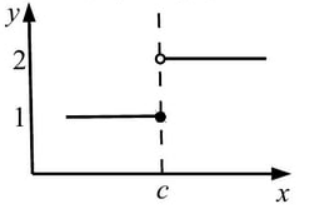
\includegraphics[width=\textwidth]{images/neprer_sleva.png}
\end{minipage}


\hypertarget{theorem_1_6}{}
\begin{theorem}
Пусть $\PP$~---~полукольцо одномерных ячеек и дана строго возрастающая функция $g: \R \rightarrow \R$ непрерывная слева. Определим $\nu_g([a, b)) = |g(b) - g(a)|$. Тогда $\nu_g$~---~счётно-аддитивная мера на полукольце ячеек.
\end{theorem}
\begin{proof}
Пусть $[a, b) = \bigcup\limits_{i = 1}^\infty [a_i, b_i)$. В силу непрерывности слева мы можем выбрать $t \in (a, b)$ такой, что $|\nu_g([a, t)) - \nu_g([a, b))| < \frac{\varepsilon}{2}$. Тогда $\forall i \in \N \ $выберем $ \delta_i: [a_i - \delta_i, b_i) \supset [a_i, b_i)$ так, чтобы $|\nu_g([a_i - \delta_i, b_i)) - \nu_g([a_i, b_i))| < \frac{\varepsilon}{2^{i + 1}}$. Тогда $[a, b) \subset \bigcup\limits_{i = 1}^\infty (a_i - \delta_i, b_i)$; $[a, t] \subset [a, b)$. По лемме Гейне-Бореля, есть некоторое конечное подпокрытие мощности $N$: $[a, t) \subset [a, t] \subset \bigcup\limits_{i = 1}^N (a_i - \delta_i, b_i) \subset \bigcup\limits_{i = 1}^N [a_i - \delta_i, b_i)$. Заметим, что конечная аддитивность, и, как следствие, конечная полуаддитивность очевидны для $\nu_g$. Значит, \[\nu_g([a, t)) \leq \sum\limits_{i = 1}^N \nu_g([a_i - \delta_i, b_i]) \leq \sum\limits_{i = 1}^N \nu_g([a_i, b_i)) + \dfrac{\varepsilon}{2} \leq \sum\limits_{i = 1}^\infty \nu_g([a_i, b_i)) + \dfrac{\varepsilon}{2}\] Но по выбору $t$: \[\nu_g([a, b)) \leq \sum\limits_{i = 1}^\infty \nu_g([a_i, b_i)) + \varepsilon\]
Поскольку $\varepsilon > 0$ было выбрано произвольно, то мы получили счётно-полуаддитивную меру на полукольце, что по ранее доказанной теореме равносильно счётно-аддитивности меры $\nu_g$.
\end{proof}
\begin{example}
Приведём пример конечно-, но не счётно-аддитивной меры. Пусть $\PP = 2^{\R^n}$. Примем $\mu(A) = 0$, если $A$~---~ограничено, и $+\infty$ иначе. Её конечная аддитивность очевидна: сумма конечного числа нулей равна 0, а если там появляется хотя бы одно неограниченное множество, то их объединение становится неограниченным. Но эта мера не является счётно-аддитивной, поскольку мы можем взять просто $\Q^n$: с одной стороны, его мера $+\infty$, поскольку оно неограниченно, а с другой стороны оно получается как счётное объединение по всем рациональным точкам. Сумма счётного числа нулей равна нулю, а следовательно его мера должна быть равна 0. Получено противоречие. Значит, мера не счётно-аддитивна.
\end{example}

\subsection{Внешняя мера}
\hypertarget{outmeasure}{}

\begin{definition}
Пусть $X$~---~абстрактное множество, а $2^X$~---~система всех его подмножеств. Функцию $\tau$: $2^X \rightarrow [0, +\infty]$ будем называть внешней мерой (по Каратеодори), если выполнены следующие условия:
\begin{enumerate}
    \item $\tau(\emptyset) = 0;$
    \item Если $A \subset \bigcup\limits_i^\infty A_i$, то $\tau(A) \leq \sum\limits_{i = 1}^\infty \tau(A_i)$.
\end{enumerate}
\end{definition}
\begin{definition}
Множество $A \subset X$ называется $\tau$-измеримым, если \[\forall E \subset X \  \text{верно, что}\  \tau(E) = \tau(E \cap A) + \tau(E \setminus A)\]
Далее будем обозначать это условие как $(*)$.
Прим. ред именно для любого множества $E$, мы как будто выбираем "пробное" множество, которое множество А аддитивно разбивает
\end{definition}

%Вот тут я не очень понял, что он имел ввиду
\begin{note}
Заметим, что для проверки условия $(*)$ достаточно проверить, что \[\tau(E) \geq \tau(E \cap A) + \tau(E \setminus A)\] для любого $E \subset X$. Обратное неравенство очевидно из 2) пункта определения внешней меры
\end{note}

%Не очень понял, что надо заменить но окей...
\begin{definition}
Обозначим $\MM_\tau$ семейство всех $\tau$-измеримых подмножеств множества $X$. \\
Очевидно, что $\emptyset, X \in \MM_\tau$.
\end{definition}

% Поясняем за символы
\begin{theorem}
Система $\MM_\tau$~---~$\sigma$-алгебра, при этом сужение $\tau$ на $\MM_\tau$, обозначается $\tau|_{\MM_\tau}$, и является счётно-аддитивной мерой на ней.
\end{theorem}
\begin{proof}
Для начала заметим, что эквивалентной записью условия измеримости является \[\tau(E) = \tau(E \cap A) + \tau(E \cap A^c)\] Значит, $\MM_\tau$ замкнута относительно операции дополнения. \\
Покажем, что система замкнута относительно объединений. Пусть $A, B \in \MM_\tau$. Пусть $E \subset X$. Тогда из измеримости $A:$ \[\tau(E) = \tau(E \cap A) + \tau(E \setminus A)\] А из измеримости $B$ мы получаем следующее: \[\tau(E \setminus A) = \tau((E \setminus A) \cap B) + \tau((E \setminus A) \setminus B)\] Таким образом, \[\tau(E) = \tau(E \cap A) + \tau((E \setminus A) \cap B) + \tau(E \setminus(A \cup B))\]
% Я, кажется, не согласен с равенством; сходу контрпример не приведу, но когда я ботал меня оно смущало, и я заменил на очевидное включение. Возможно, равенство есть, но, кажется, включения хватает для доказательства теоремы.
В тоже время, поскольку $(E \cap A) \cup ((E \setminus A) \cap B) \supset E \cap (A \cup B)$, то \[\tau(E) \geq \tau(E \cap (A \cup B)) + \tau(E \setminus (A \cup B))\] Таким образом, мы показали, что $\MM_\tau$~---~алгебра с единицей $X$. \\
Покажем, что $\tau$ является конечно-аддитивной мерой на этой алгебре. Зафиксируем $A, B \in \MM_\tau$ такие, что $A \cap B = \emptyset$. Тогда из измеримости $A$ следует, что при $E = A \sqcup B$ выполняется следующее \[\tau(A \sqcup B) = \tau((A \sqcup B) \cap A) + \tau((A \sqcup B) \setminus A) = \tau(A) + \tau(B)\] Что нам и требовалось показать. Теперь по индукции это продолжается для произвольного числа дизъюнктных множеств алгебры. \\
Докажем даже более сильную версию конечной аддитивности. Заметим, что
\[(E \cap (A \sqcup B)) \cap A = E \cap A\]
\[(E \cap (A \sqcup B)) \setminus A = E \cap B\]
А значит, поскольку $A \sqcup B \in \MM_\tau$, то \[\tau(E \cap (A \sqcup B)) = \tau((E \cap (A \sqcup B)) \cap A) + \tau((E \cap (A \sqcup B)) \setminus A) = \tau(E \cap A) + \tau(E \cap B)\]
Поэтому верно следующее утверждение. Для $\forall E \subset X$ и для $\forall$ дизъюнктной системы $\{A_i\}_{i = 1}^N$ справедливо такое равенство: \[\tau(E \cap (\bigsqcup\limits_{i = 1}^N A_i)) = \sum\limits_{i = 1}^N \tau(E \cap A_i)\]
С другой стороны, поскольку любая алгебра является полукольцом, и $\tau$~---~счётно-полуаддитивная мера на $\MM_\tau$, то мы получаем что $\tau$~---~счётно-аддитивная мера на $\MM_\tau$. \\ 
Теперь покажем, что $\MM_\tau$~---~$\sigma$-алгебра. \\ Пусть $\{A_i\}_{i = 1}^\infty \subset \MM_\tau$ и $A_i \cap A_j = \emptyset$ если $i \neq j$. Пусть $A = \bigsqcup\limits_{i = 1}^\infty A_i$. Заметим, что из того, что наша система множеств является алгеброй, следует для $\forall E \subset X$ \[\tau(E) = \tau(E \cap (\bigsqcup\limits_{i = 1}^n A_i)) + \tau(E \setminus (\bigsqcup\limits_{i = 1}^n A_i)) = \sum\limits_{i = 1}^n \tau(E \cap A_i) + \tau(E \setminus \bigsqcup_{i = 1}^n A_i) \geq\]
\[\geq \sum\limits_{i = 1}^n \tau(E \cap A_i) + \tau(E \setminus \bigsqcup\limits_{i = 1}^\infty A_i)\]
Поскольку это верно для произвольного $n \in \N$, то, взяв $\sup$ по $n \in \N$, мы получаем \[\tau(E) \geq \sum\limits_{i = 1}^\infty \tau(E \cap A_i) + \tau(E \setminus \bigsqcup\limits_{i = 1}^\infty A_i) \geq \tau(E \cap \bigsqcup A_i) + \tau(E \setminus \bigsqcup A_i)\]
Значит, $A$~---~измеримое. \\
Пусть теперь $A_i$ не обязательно дизъюнктные. Тогда определив $A_n' = A_n \setminus \bigcup\limits_{i = 1}^{n-1} A_i$, мы получим последовательность дизъюнктных $\{A_i'\}$ с тем же объединением. Поскольку это объединение лежит в алгебре, то мы получаем, что $\MM_\tau$~---~$\sigma$-алгебра.
\end{proof}
\begin{theorem}
Конечно-аддитивная мера $\mu$ на $\sigma$-алгебре $\MM$ является счётно-аддитивной $\Longleftrightarrow$ $\mu$ непрерывна снизу, то есть для последовательности $\{ A_i\} \subset \MM$: $A_i \subset A_{i + 1}$ и $A = \bigcup\limits_{i = 1}^{+\infty} A_i \hookrightarrow \mu(A) = \lim\limits_{k \rightarrow \infty} \mu(A_k)$.
\end{theorem}
\begin{proof}
($\Longrightarrow$) Пусть $\mu$~---~счётно-аддитивна. Тогда поскольку $\MM$~---~$\sigma$-алгебра, то определив $A_1' := A_1, A_n' := A_n \setminus A_{n - 1} \forall n \in \N$ мы получим дизъюнктную последовательность множеств с тем же объединением. Тогда \[\mu(A) = \mu(\bigsqcup\limits_{n = 1}^\infty A_n') = \sum\limits_{n = 1}^\infty \mu(A_n') = \lim\limits_{N \rightarrow \infty} \sum\limits_{n = 1}^N \mu(A_n') = \lim\limits_{N \rightarrow \infty} \mu(A_N)\]
    \begin{minipage}{\textwidth}
    \centering
    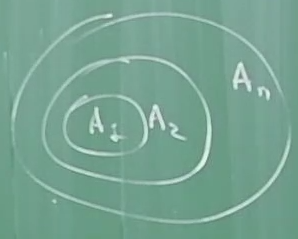
\includegraphics[width=0.35\textwidth]{images/Screenshot_5.png} 
    \end{minipage}
    \textit{Схематическое описание множеств, непрерывных снизу, где кольца между $A_k$ и $A_{k+1}$ это $A_{k+1}'$}


% тут кажется что-то ещё надо починить
($\Longleftarrow$) Пусть $\mu$~---~непрерывна снизу. Хотим получить счетную аддитивность. Тогда если мы возьмём произвольную последовательность дизъюнктных множеств $\{A_i\}_{i = 1}^\infty$ и определим $F_k = \bigsqcup\limits_{i = 1}^k A_i$ для каждого $k \in \N$, то мы получим искомую монотонную последовательность множеств $F_k \subset F_{k+1}$.  Из конечной аддитивности меры $\mu(F_k) = \sum\limits_{i = 1}^k \mu (A_i)$. Отсюда и из непрерывности меры следует, что $\exists \lim\limits_{k \rightarrow \infty} \sum\limits_{i = 1}^k \mu (A_i) = \sum\limits_{i = 1}^{+\infty} \mu (A_i) = \mu(A)$
\end{proof}